\chapter{Limitations actuelles}\label{ch:limitations-actuelles}

De nombreux facteurs rendent l'utilisation d'ordinateurs quantiques pour le moment inutile
hors de la recherche, et même certains spécialistes ne sont pas convaincus qu'on arrive à
passer outre afin de rendre cette technologie utilisable, et cela demeure un grand débat
dans la communauté scientifique.
Certains points sont purement liés aux algorithmes que l'on désire implémenter et qui serait
potentiellement irréalisable en pratique, et d'autres concernent en général l'implémentation
physique des ordinateurs quantiques, ainsi que certaines considérations purement humaines.\\ \\
Ces dernières sont les plus évidentes, et sont plus générale au sujet des nouvelles technologies.
En effet, comme de nombreux autres outils électroniques, tels que les téléphones portables,
ordinateurs, certaine télévision récente et ainsi de suite, les ordinateurs quantiques
nécessitent dans leurs fabrications actuelles l'utilisation de matériaux qui sont utiles dans
quantité de secteur, mais ne sont pas illimité sur notre planète.
Les plus évidents seront le silicium, utilisé dans n'importe quel processeur actuel, et
qui est la base de la plupart des processeurs quantique actuel, comme évoqué dans la section
hardware.
D'autre part, l'isolation thermique d'un ordinateur quantique est généralement composé d'or
(voir illustration en figure~\ref{fig:photo-qc}), qui est également très prisé dans le reste
de l'industrie pour ses multiples avantages d'un point de vue esthétique, thermique ou électronique.

\begin{figure}[H]
\centering
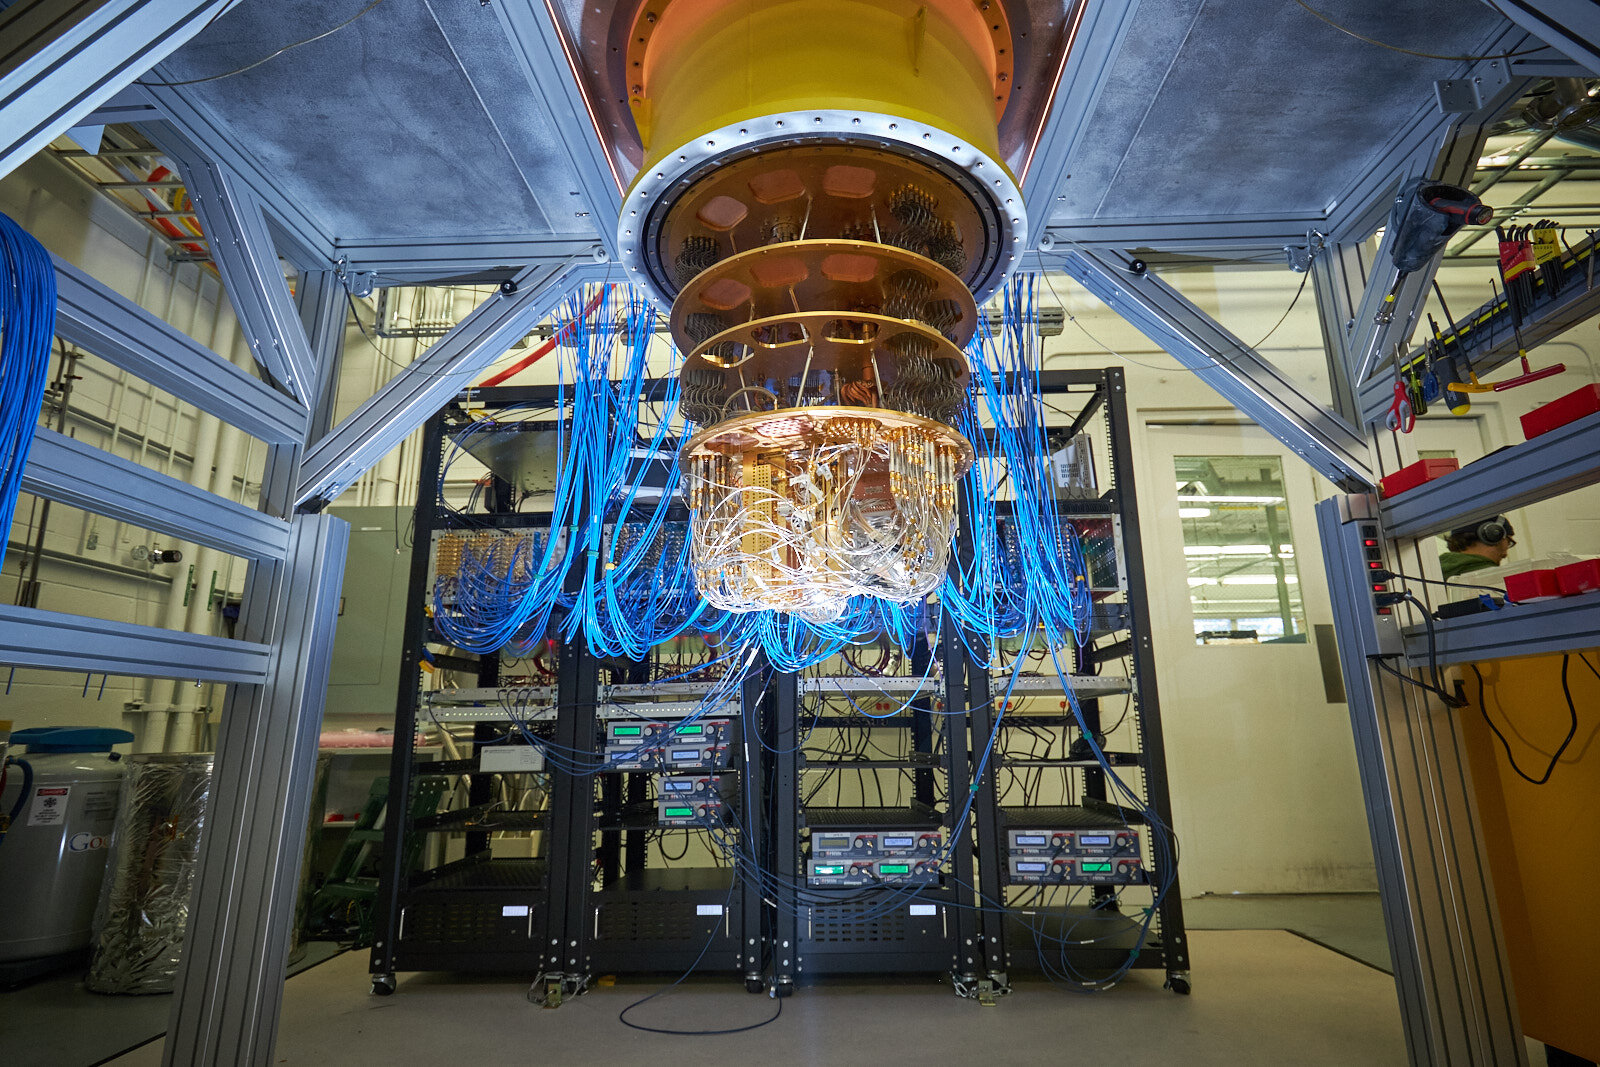
\includegraphics[width=0.7\textwidth]{images/futur/limitation/qpu.eps}
\caption{Photo d'un ordinateur quantique, credit : Rocco Ceslin}
\label{fig:photo-qc}
\end{figure}

De plus, une considération de l'ordre environnementale entre aussi en compte.
Tout comme la question se pose dans le cadre de l'intelligence artificiel, l'utilisation en
énergie des ordinateurs quantiques ne serait vraisemblablement pas négligeable.
En effet, ils nécessitent un isolement total ou presque du monde extérieur afin de fonctionner,
ce qui demande outre l'isolation matérielle évoquée plus tôt, également un refroidissement à des
températures proches du zéro absolu, qui est un processus très demandeur en énergie.
Si l'on discute plus précisément des qubits supraconducteurs déjà présentés précédemment, il ne
suffit pas juste de les mettre dans un gros congélateur, car on les contrôle depuis l'extérieur.
Cela fait qu'il faut faire passer les signaux électromagnétiques depuis l'air à température ambiante
jusqu'au processeur quantique au zéro absolu, tout en gardant une bonne qualité de signal.
Il faut donc le refroidir petit à petit et corriger les erreurs sur le signal, tout des processus
nécessitant de l'énergie et des méthodes industriels de pointe pour le fabriquer.\\ \\
Il y a ensuite tous les doutes liés à la technologie à proprement parlé.
Tout d'abord, comme ce fut déjà évoqué plus tôt, les ordinateurs quantiques sont soumis à
beaucoup d'erreur dans les résultats dû à de multiples facteurs.
Ce sont déjà des aspects théoriques menant à une réalisation complexe.
Dans un ordinateur classique, un bit est par exemple une quantité de charge électrique, qui est
tout à fait maitrisable et peu sensible à l'environnement, même s'il y a en pratique toujours
quelques défaillances matérielles.
De l'autre côté, un ordinateur quantique est fondamentalement un système quantique que l'on
considère comme isolé, mais ce n'est concrètement pas possible.
De fait, malgré la grande isolation thermique, radiative et électromagnétique, il y aura toujours
des petites perturbations venant de l'extérieur, et qui peut impacter n'importe quel partie du
système, que ce soit les qubits, les portes logiques ou les mesures.
Cette nécessité d'isolation s'explique, car l'interaction par exemple avec des photons sera
d'un point de vue de la mécanique quantique une mesure, et donc un effondrement de la fonction
d'onde, ce qui fait que l'on perd l'état que l'on a construit et que l'on désirait utiliser.
Dans la même veine, la calibration des portes logiques est un processus complexe, car il faut
faire les calculs théoriques pour chaque qubit et chaque porte, et les ajuster en fonction des
mesures faites sur le système, et ce calibrage doit être fait régulièrement afin que tout reste
fonctionnel.\\
Néanmoins, plusieurs solutions sont envisagées pour pallier ces problèmes~\cite{error-code}.
Sur un ordinateur classique, on utilise des codes correcteurs d'erreurs pour pallier les erreurs
de transmission.
Le plus simple classiquement et de copier plusieurs fois le message, et de prendre la majorité
des résultats pour obtenir le bon message.
Mais il y en a d'autres, comme le code de Hamming, qui permet de détecter et corriger une erreur
dans un mot binaire ou celui de Golay, qui permet de détecter et corriger jusqu'à trois erreurs.
On essaie de faire de même pour les ordinateurs quantiques, mais cela est plus complexe, car
il faut arriver à corriger tout l'état du système, et pas juste un 0 ou un 1.
De plus, il y a le théorème de non-clonage, qui dit que l'on ne peut pas copier un état quantique
qui rend impossible la méthode simple de copier tel quel le système pour le comparer et corriger.
Une des méthodes les plus prometteuses est le \textit{code de surface}~\cite{surface-code}, qui utilise un réseau de
qubits physiques pour stocker un qubit logique, et qui peut être agrandi pour être plus résistant.
Néanmoins, pour être utilisable, il faut que l'ordinateur soit construit avec les qubits disposés
selon l'architecture nécessaire pour le code de surface.
Le principe de ce code est de vérifier chaque qubit avec ses voisins, et bloquant ainsi les
possibilités d'évolution du système.
Afin de pouvoir utiliser un qubit logique, on fait un ``trou'' dans le réseau de qubits physiques
qui permettra d'offrir un degré de liberté pour pouvoir faire évoluer le système.\\
D'autres méthodes sont également mise en place, comme celle utilisée dans ce travail, qui consiste
en l'exécution de l'algorithme plusieurs fois et de voir quel est le résultat le plus probable,
ce qui peut être optimisé par des méthodes statistiques si l'on connaît les erreurs de mesure
des différents qubits par exemple.
Il y a également des méthodes qui sont directement dans la construction de l'ordinateur, comme
les \textit{qubits de chat}~\cite{Lescanne2020}, qui sont des qubits qui sont fabriqués de telle sorte
à s'auto-corriger.

\begin{figure}[H]
\centering
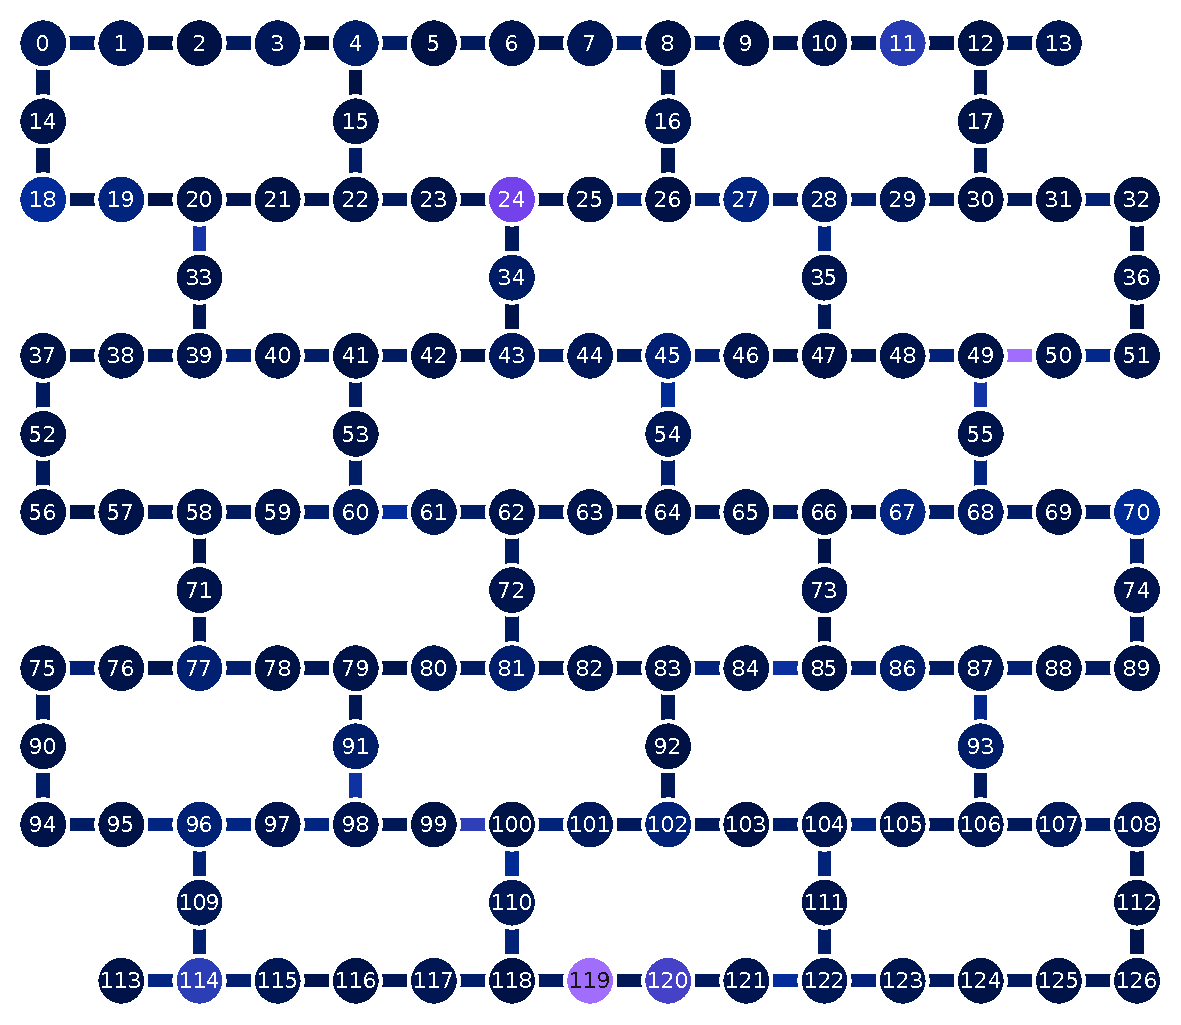
\includegraphics[width=0.7\textwidth]{images/futur/limitation/ibm_brisbane_example.eps}
\caption{Exemple d'architecture d'un ordinateur quantique ($ibm\_brisbane$), les cercle représente les qubits (plus sombre est plus précis dans la mesure) et les liaisons entre eux (plus sombre a moins d'erreur sur la $CZ$)}
\label{fig:arch-qc}
\end{figure}

L'architecture d'un ordinateur quantique est en elle-même un enjeu majeur.
En effet, il faut pouvoir et contrôler les qubits suffisamment simplement sans perdre en fiabilité,
mais également réfléchir aux futurs moyens d'augmenter le nombre de qubits.
En effet, un arrangement peut être pratique pour une centaine de qubits, mais impossible sur des
milliers.
De plus, comme on le voit sur la figure \ref{fig:arch-qc}, sur un ordinateur quantique actuelle,
tous les qubits ne sont pas liée entre eux, donc lorsque qu'on conçoit un circuit en théorie en
faisant des superpositions par des portes par exemples $CX$ sur n'importe quel qubits, en pratique
pour en exécuter une entre le qubit 26 et 35 il faudrait passer par des opérations sur ceux 27 et
28 ce qui complique la mise en place.
Notons également que l'on voit sur cette figure que les divers éléments (porte $CZ$, qubits) n'ont
pas la même fiabilité et que cela doit en plus être régulièrement calibré.\\ \\
%%%%%%%%%%%%%%% BlaBla sur les sources d'erreur (environnement, hamiltonien, architecture) + méthode pour passer outre (surface code avec comparaison à un code classique, conception - cf. qubit du chat par exemple) %%%%%%%%%%%%%%%
Finalement, il y a les limites propres au paradigme.
En effet, on suppose par exemple que la classe des problèmes solubles en temps polynomiale par
un ordinateur quantique est plus grande que celle d'un ordinateur classique.
Mais dire cela ainsi est quelque peu mensonger, car on considère traditionnellement comme classe
polynomiale pour les ordinateurs quantiques la complexité dite $BQP$
(\textit{bounded-error quantum polynomial time}), qui signifie qu'un problème peut être résolu
dans un temps polynomial avec une erreur inférieur à $\frac{1}{3}$.
Il existe un groupe de complexité similaire pour les ordinateurs classiques, nommée $BPP$
(\textit{bounded-error probabilistic polynomial time}), mais elle est moins intéressante,
car c'est un système bien déterminé et demeure selon nos connaissances actuelles une moins
grande catégorie de problèmes~\cite{wiki:bqp}.\\
L'algorithme de Shor est un bon exemple d'un problème qui n'est vraisemblablement pas dans
$P$ (temps polynomial) mais qui est dans $BQP$.
Comme on a vu avec celui-ci, on n'est pas certain d'obtenir le bon résultat à la mesure, ce qui
fait que par manque de chance, en pratique, cela pourrait prendre plus de temps qu'un algorithme
en général plus lent, mais qui donne à coup sûr la solution escomptée.
Si l'on rajoute ce qui a été discuté plus haut au sujet du bruit et des erreurs, cela rend les
ordinateurs quantiques encore plus complexes à mettre en place comme il faut trouver des applications
ne subissant pas trop ces erreurs.\\
Citons encore certaines méthodes pour lesquels les ordinateurs quantiques peuvent être avantageux,
comme pour du \textit{machine learning}, où pour bénéficier d'une accélération le circuit doit être
assez grand.
Néanmoins, plus le circuit grandit, plus la préparation de l'état du système quantique nécessaire à
la réalisation de l'algorithme devient compliqué et remet donc en question l'avantage.
On arrive ainsi à un cercle vicieux pour lequel l'avantage est incertain, car plus le problème est
gros plus l'avantage est conséquent, mais plus la mise en place est compliquée et en réduit quelque
peu l'intérêt~\cite{McClean2018}.\\ \\
En résumé, il n'y a encore aucune certitude sur la viabilité de la technologie, même s'il y a de
nombreux signes encourageants.
Toutes ces limitations présentent des défis qui devront être contourné ou outrepasser à l'avenir
grâce aux débouchés de la recherche.
